\documentclass{beamer}
\usepackage{amsmath}
\usepackage{hyperref}
\usepackage{listings}
\usepackage{xcolor}
\hypersetup{colorlinks=true, citecolor=blue, filecolor=blue, linkcolor=blue, urlcolor=blue}
\definecolor{codegreen}{rgb}{0,0.6,0}
\definecolor{codegray}{rgb}{0.5,0.5,0.5}
\definecolor{codepurple}{rgb}{0.58,0,0.82}
\definecolor{backcolour}{rgb}{0.95,0.95,0.92}
 
\lstdefinestyle{mystyle}{
    backgroundcolor=\color{backcolour},   
    commentstyle=\color{codegreen},
    keywordstyle=\color{magenta},
    numberstyle=\tiny\color{codegray},
    stringstyle=\color{codepurple},
    basicstyle=\ttfamily\footnotesize,
    breakatwhitespace=false,         
    breaklines=true,                 
    captionpos=b,                    
    keepspaces=true,                 
    %numbers=left,                    
    numbersep=5pt,                  
    showspaces=false,                
    showstringspaces=false,
    showtabs=false,                  
    tabsize=2
}
 
\lstset{style=mystyle}

\mode<presentation> {

% The Beamer class comes with a number of default slide themes
% which change the colors and layouts of slides. Below this is a list
% of all the themes, uncomment each in turn to see what they look like.

%\usetheme{default}
\usetheme{AnnArbor}
%\usetheme{Antibes}
%\usetheme{Bergen}
%\usetheme{Berkeley}
%\usetheme{Berlin}
%\usetheme{Boadilla}
%\usetheme{CambridgeUS}
%\usetheme{Copenhagen}
%\usetheme{Darmstadt}
%\usetheme{Dresden}
%\usetheme{Frankfurt}
%\usetheme{Goettingen}
%\usetheme{Hannover}
%\usetheme{Ilmenau}
%\usetheme{JuanLesPins}
%\usetheme{Luebeck}
%\usetheme{Madrid}
%\usetheme{Malmoe}
%\usetheme{Marburg}
%\usetheme{Montpellier}
%\usetheme{PaloAlto}
%\usetheme{Pittsburgh}
%\usetheme{Rochester}
%\usetheme{Singapore}
%\usetheme{Szeged}
%\usetheme{Warsaw}

% As well as themes, the Beamer class has a number of color themes
% for any slide theme. Uncomment each of these in turn to see how it
% changes the colors of your current slide theme.

%\usecolortheme{albatross}
%\usecolortheme{beaver}
%\usecolortheme{beetle}
%\usecolortheme{crane}
%\usecolortheme{dolphin}
%\usecolortheme{dove}
%\usecolortheme{fly}
%\usecolortheme{lily}
%\usecolortheme{orchid}
%\usecolortheme{rose}
%\usecolortheme{seagull}
%\usecolortheme{seahorse}
%\usecolortheme{whale}
%\usecolortheme{wolverine}

%\setbeamertemplate{footline} % To remove the footer line in all slides uncomment this line
\setbeamertemplate{footline}[page number] % To replace the footer line in all slides with a simple slide count uncomment this line

\setbeamertemplate{navigation symbols}{} % To remove the navigation symbols from the bottom of all slides uncomment this line
}

\usepackage{graphicx} % Allows including images
\usepackage{booktabs} % Allows the use of \toprule, \midrule and \bottomrule in tables
%\usepackage {tikz}
\usepackage{tkz-graph}
\GraphInit[vstyle = Shade]
\tikzset{
  LabelStyle/.style = { rectangle, rounded corners, draw,
                        minimum width = 2em, fill = yellow!50,
                        text = red, font = \bfseries },
  VertexStyle/.append style = { inner sep=5pt,
                                font = \normalsize\bfseries},
  EdgeStyle/.append style = {->, bend left} }
\usetikzlibrary {positioning}
%\usepackage {xcolor}
\definecolor {processblue}{cmyk}{0.96,0,0,0}
%----------------------------------------------------------------------------------------
%	TITLE PAGE
%----------------------------------------------------------------------------------------

\title[Probabilistic Surrogate Models]{Numerical Optimization 15: Probabilistic Surrogate Models} %

\author{Qiang Zhu} % Your name
\institute[University of Nevada Las Vegas] % Your institution as it will appear on the bottom of every slide, may be shorthand to save space
{
University of Nevada Las Vegas\\ % Your institution for the title page
\medskip
}
\date{\today} % Date, can be changed to a custom date

\begin{document}

\begin{frame}
\titlepage % Print the title page as the first slide
\end{frame}

\begin{frame}
\frametitle{Overview} % Table of contents slide, comment this block out to remove it
\tableofcontents % Throughout your presentation, if you choose to use \section{} and \subsection{} commands, these will automatically be printed on this slide as an overview of your presentation
\end{frame}

%----------------------------------------------------------------------------------------
%	PRESENTATION SLIDES
%----------------------------------------------------------------------------------------

%------------------------------------------------

\section{Gaussian Distribution}
\begin{frame}{Gaussian Distribution}
In surrogate modeling, a strategy is to use a probabilistic model to estimate the confidence of the model, one of which is Gaussian process.

An $n$-dimensional Gaussian distribution is parameterized by its mean $\mu$ and its covariance matrix $\Sigma$. The probability density at $\boldsymbol{x}$ is
\begin{equation*}
    \mathcal{N}(\boldsymbol{x}|\boldsymbol{\mu}, \boldsymbol{\Sigma}) =
    (2\pi)^{-n/2} |\boldsymbol{\Sigma}|^{-1/2} \exp\bigg(-\frac{1}{2}(\boldsymbol{x-\mu})^T \boldsymbol{\Sigma}^{-1}(\boldsymbol{x-\mu})\bigg)
\end{equation*}

\begin{figure}
\centering
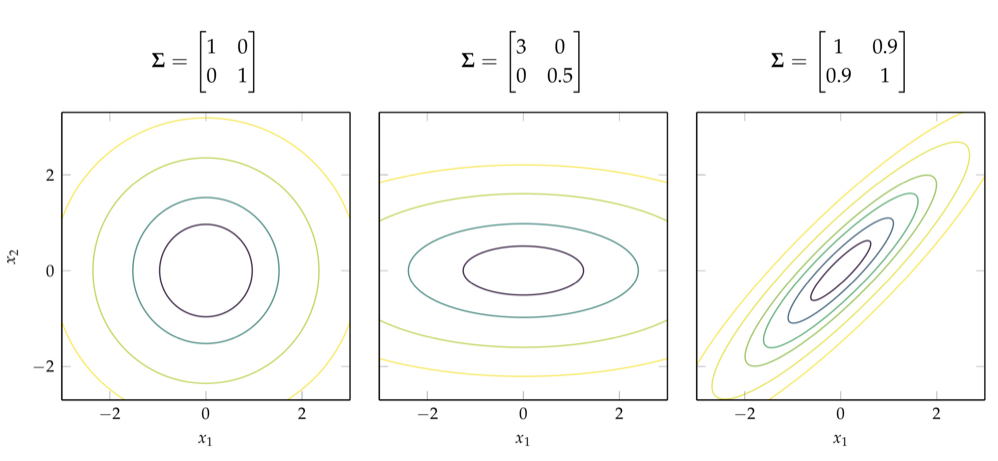
\includegraphics[width=100mm]{Figs/gaussian.jpeg}
\end{figure}   

\end{frame}

\begin{frame}{Gaussian Distribution: Nice Properties}
A value sampled from a Gaussian is written 
\begin{equation*}
    \boldsymbol{x} \sim \mathcal{N}(\boldsymbol{\mu}, \boldsymbol{\Sigma})
\end{equation*}

Two jointly Gaussian random variables $\boldsymbol{a}$ and $\boldsymbol{b}$ can be written
\begin{equation*}
    \begin{bmatrix} 
    \boldsymbol{a}\\
    \boldsymbol{b}
    \end{bmatrix}
    \sim \mathcal{N}\bigg(
    \begin{bmatrix}
    \boldsymbol{\mu}_a \\
    \boldsymbol{\mu}_b
    \end{bmatrix},
    \begin{bmatrix}
    \boldsymbol{A}, &\boldsymbol{C} \\
    \boldsymbol{C}^T,& \boldsymbol{B}
    \end{bmatrix}
    \bigg)
\end{equation*}

where the marginal distribution for a vector of random variables is given by its corresponding mean and covariance
\begin{equation*}
    \boldsymbol{a} \sim \mathcal{N}(\boldsymbol{\mu}_a, \boldsymbol{A}) ~~~~~~~~~~
    \boldsymbol{b} \sim \mathcal{N}(\boldsymbol{\mu}_b, \boldsymbol{B}) 
\end{equation*}

The \textcolor{blue}{conditional distribution} for a multivariate Gaussian also has a convenient closed-form solution:
\begin{equation*}
\begin{split}
    \boldsymbol{a} | \boldsymbol{b} & \sim \mathcal{N}(\boldsymbol{\mu}_{a|b}, \boldsymbol{\Sigma}_{a|b}) \\ 
    \boldsymbol{\mu}|_{a|b} &= \boldsymbol{\mu}_{a} + \boldsymbol{CB}^{-1}(\boldsymbol{b} - \boldsymbol{\mu}_{a})\\
    \boldsymbol{\Sigma}_{a|b} &= \boldsymbol{A} − \boldsymbol{CB}^{−1}\boldsymbol{C}^⊤    
\end{split}
\end{equation*}

\end{frame}

\section{Gaussian Processes}
\begin{frame}{Gaussian Processes}
A special type of surrogate model known as a Gaussian process allows us not only to predict $f$ but also to quantify our uncertainty in that prediction using a probability distribution.

\begin{equation*}
    \begin{bmatrix} 
    y_1\\
    \vdots\\
    y_m\\
    \end{bmatrix}
    \sim \mathcal{N}\bigg(
    \begin{bmatrix}
    m(x_1) \\
    \vdots \\
    m(x_m)
    \end{bmatrix},
    \begin{bmatrix}
    k(x_1, x_1) & \cdots & k(x_1, x_m)\\
    \vdots & \ddots & \vdots \\
    k(x_m, x_1) & \cdots & k(x_m, x_m)\\
    \end{bmatrix}
    \bigg)
\end{equation*}

where 
\begin{itemize}
    \item $m(x)$ is the mean function to represent the prior knowledge about the function
    \item $k(x, x`)$ is the covariance function to control the smoothness.
\end{itemize}

\end{frame}

\begin{frame}{Kernel Function}
Kernel function is to control the smoothness of the sample. A common choice of $k$ is the squared exponential function
\begin{equation*}
    k(x, x`) = \exp\bigg(-\frac{(x-x`)^2}{2l^2}\bigg)
\end{equation*}

\begin{figure}
\centering
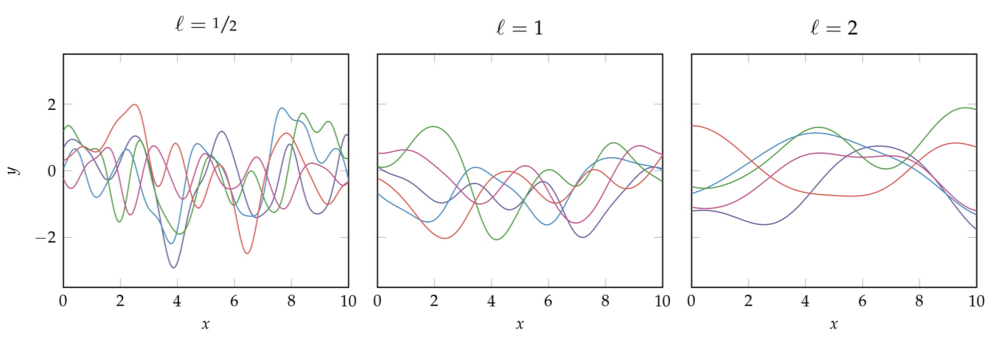
\includegraphics[width=120mm]{Figs/kernel.jpeg}
\end{figure}  


\end{frame}

\section{Prediction}
\begin{frame}{Prediction}
Suppose we already have a set of points $X$ and the corresponding $\boldsymbol{y}$, we wish to predict the values $\hat{\boldsymbol{y}}$ at points $X^*$. from the joint distribution
\begin{equation*}
    \begin{bmatrix} 
    \hat{y}\\
    y\\
    \end{bmatrix}
    \sim \mathcal{N}\bigg(
    \begin{bmatrix}
    \boldsymbol{m}(X^*) \\
    \boldsymbol{m}(X)
    \end{bmatrix},
    \begin{bmatrix}
    \boldsymbol{K}(X^*, X^*)  & \boldsymbol{K}(X^*, X)\\
    \boldsymbol{K}(X, X^*)    & \boldsymbol{K}(X, X)\\
    \end{bmatrix}
    \bigg)
\end{equation*}

In the equation above, we use the functions $m$ and $K$, which are defined as follows:
\begin{equation*}
\begin{split}
\boldsymbol{m}(X) &= [m(\boldsymbol{x}^1), \cdots, m(\boldsymbol{x}^n)]\\
\boldsymbol{K}(X, X`) & = 
    \begin{bmatrix}
    k(X^*, X^*) & \cdots & k(X^*, X)\\
    \vdots & \ddots & \vdots \\
    k(X, X^*)  &\cdots  & k(X, X)
    \end{bmatrix}
\end{split}
\end{equation*}

The conditional distribution is given by: $\hat{\boldsymbol{y}} | \boldsymbol{y} \sim \mathcal{N}(\boldsymbol{\mu}^*, \boldsymbol{\Sigma}^*)$
\begin{equation*}
\begin{split}
    \boldsymbol{\mu}^* &= m(X^{∗}) +  K(X^{∗}, X) K(X, X)^{-1} (\boldsymbol{y} - m(X)) \\
    \boldsymbol{\Sigma}^* &= K(X^{*} - X^{*}) - K(X^{∗}, X)K(X, X)^{-1}K(X, X^{*}))    
\end{split}
\end{equation*}


\end{frame}

\section{Gradient Measurements}
\begin{frame}{Gradient Measurements}
Gradient observations can be incorporated into Gaussian processes in a manner consistent with the existing Gaussian process machinery.
\begin{equation*}
    \begin{bmatrix} 
    y\\
    \nabla y\\
    \end{bmatrix}
    \sim \mathcal{N}\bigg(
    \begin{bmatrix}
    \boldsymbol{m}(f) \\
    \boldsymbol{m}(\nabla)
    \end{bmatrix},
    \begin{bmatrix}
    \boldsymbol{K}_{ff}  & \boldsymbol{K}_{f\nabla}\\
    \boldsymbol{K}_{\nabla f}    & \boldsymbol{K}_{\nabla \nabla}\\
    \end{bmatrix}
    \bigg)
\end{equation*}
Where
\begin{itemize}
    \item  $y\sim N(m_f, K_{ff})$ is a traditional Gaussian process, 
    \item $\boldsymbol{m\nabla}$ is a mean function for the gradient,
    \item $\boldsymbol{K}_{f\nabla}$ is the covariance matrix between function values and gradients, 
    \item $\boldsymbol{K}_{\nabla f}$ is the covariance matrix between function gradients and values, 
    \item $\boldsymbol{K}_{\nabla \nabla}$ is the covariance matrix between function gradients.
\end{itemize}
\end{frame}

\begin{frame}{Prediction}
    Prediction can be accomplished in the same manner as with a traditional Gaussian process. We first construct the joint distribution
\begin{equation*}
    \begin{bmatrix} 
    \hat{y}\\
    y\\
    \nabla y\\
    \end{bmatrix}
    \sim \mathcal{N}\bigg(
    \begin{bmatrix}
    \boldsymbol{m}(f(X^*)) \\
    \boldsymbol{m}(f(X)) \\
    \boldsymbol{m}(\nabla X)
    \end{bmatrix},
    \begin{bmatrix}
    \boldsymbol{K}_{ff}(X^*, X^*)     &\boldsymbol{K}_{ff}(X^*, X)  & \boldsymbol{K}_{f\nabla}(X^*, X)\\
    \boldsymbol{K}_{ff}(X, X^*)       &\boldsymbol{K}_{ff}(X, X)  & \boldsymbol{K}_{f\nabla}(X, X)\\
    \boldsymbol{K}_{\nabla f}(X, X^*) &\boldsymbol{K}_{\nabla f}(X, X) & \boldsymbol{K}_{\nabla \nabla}(X, X)\\
    \end{bmatrix}
    \bigg)
\end{equation*}

The conditional distribution follows the same Gaussian relations

\begin{equation*}
{\tiny 
%{\small
\begin{split}
    \boldsymbol{\mu}^* &= m_f(X^{∗}) +  
    \begin{bmatrix}
        K_{ff}(X^{∗}, X) \\
        K_{\nabla f} (X^{∗}, X)
    \end{bmatrix}
    ^T
    \begin{bmatrix}
        K_{ff}(X, X)& K_{f\nabla}(X, X)\\
        K_{\nabla f}(X, X) & K_{\nabla\nabla}(X, X)
    \end{bmatrix}
    ^{-1}
    \begin{bmatrix}
        \boldsymbol{y} - m(X) \\
        \nabla \boldsymbol{y} - m\nabla (X)     
    \end{bmatrix}
\\
    \boldsymbol{\Sigma}^* &= K_ff(X^{*} - X^{*}) - 
    \begin{bmatrix}
        K_{ff}(X^{∗}, X) \\
        K_{\nabla f} (X^{∗}, X)
    \end{bmatrix}
    ^T  
    \begin{bmatrix}
        K_{ff}(X, X)& K_{f\nabla}(X, X)\\
        K_{\nabla f}(X, X) & K_{\nabla\nabla}(X, X)
    \end{bmatrix}
    ^{-1}
    \begin{bmatrix}
        K_{ff}(X^{∗}, X) \\
        K_{\nabla f} (X^{∗}, X)
    \end{bmatrix}
\end{split}
}
\end{equation*}    


\end{frame}

\section{Noisy Measurements}
\begin{frame}{Noisy Measurements}
So far we have assumed that the objective function $f$ is deterministic. In practice, however, evaluations of $f$ may include measurement noise,
experimental error. We can model noisy evaluations as $y = f (x) + z$, where $z$ is zero-mean Gaussian noise, \textcolor{blue}{$z \sim \mathcal{N}(0, v)$}. The new joint distribution is:
\begin{equation*}
    \begin{bmatrix} 
    \hat{y}\\
    y\\
    \end{bmatrix}
    \sim \mathcal{N}\bigg(
    \begin{bmatrix}
    \boldsymbol{m}(X^*) \\
    \boldsymbol{m}(X)
    \end{bmatrix},
    \begin{bmatrix}
    \boldsymbol{K}(X^*, X^*)  & \boldsymbol{K}(X^*, X)\\
    \boldsymbol{K}(X, X^*)    & \boldsymbol{K}(X, X) + \textcolor{blue}{v{\bf I}}\\
    \end{bmatrix}
    \bigg)
\end{equation*}

The conditional distribution is given by: $\hat{\boldsymbol{y}} | \boldsymbol{y}  \sim \mathcal{N}(\boldsymbol{\mu}^*, \boldsymbol{\Sigma}^*)$
\begin{equation*}
\begin{split}
    \boldsymbol{\mu}^* &= m(X^{∗}) +  K(X^{∗}, X) (K(X, X)+ \textcolor{blue}{v{\bf I}})^{-1} (\boldsymbol{y} - m(X)) \\
    \boldsymbol{\Sigma}^* &= K(X^{*} - X^{*}) - K(X^{∗}, X)(K(X, X)+\textcolor{blue}{v{\bf I}})^{-1}K(X, X^{*}))    
\end{split}
\end{equation*}


\end{frame}

\section{Fitting Gaussian Processes}
\begin{frame}{Fitting Gaussian Processes}
Given a dataset with $n$ entries, the log likelihood is given by
\begin{equation*}
\begin{split}
    \log p(\boldsymbol{y}|X, v, \boldsymbol{\sigma}) =& 
    -\frac{n}{2}\log{2\pi} - \frac{1}{2}\log |\boldsymbol{K}_\theta(X, X) + v\boldsymbol{I}|\\
    &-\frac{1}{2}(\boldsymbol{y}-\boldsymbol{m}_\theta)^T (\boldsymbol{K}_\theta(X, X) + v\boldsymbol{I})^{-1}
    y-\boldsymbol{m}_\theta(X)    
\end{split}
\end{equation*}
The gradient is then given by
\begin{equation*}
\begin{split}
    \frac{\partial}{\partial \theta} \log p(\boldsymbol{y}|X, v, \boldsymbol{\sigma}) =
    \frac{1}{2}\boldsymbol{y}^T \boldsymbol{K}^{-1} \frac{\partial \boldsymbol{K}}{\theta_j} \boldsymbol{K}^{-1} \boldsymbol{y}
    - \frac{1}{2}\textrm{Tr}\bigg(\boldsymbol{\Sigma}^{-1}_{\theta} \frac{\partial \boldsymbol{K}}{\theta_j} \bigg)
\end{split}
\end{equation*}

where $\boldsymbol{\Sigma}^{-1}_{\theta} = \boldsymbol{K}_\theta(X, X) + v{\bf I}$

\end{frame}


\section{Summary}
\begin{frame}{Summary}
    \begin{itemize}
        \item Gaussian processes are probability distributions over functions.
        %\item The choice of kernel affects the smoothness of the functions sampled from a Gaussian process.
        \item The multivariate normal distribution has analytic conditional and marginal distributions.
        \item We can compute the mean and standard deviation of our prediction of an objective function at a particular design point given a set of past evaluations.
        \item We can incorporate gradient observations to improve our predictions of the objective value and its gradient.
        \item We can incorporate measurement noise into a Gaussian process.
        \item We can fit the parameters of a Gaussian process using maximum likelihood.
    \end{itemize}
\end{frame}
\end{document}

